The logistic model assumes that the probability of outcome follows a logistic curve from 1 (at low covariate values assuming a protective covariate) to 0 (at high covariate values). If there is only one covariate which is the antibody titre measurement, then the model is:

\begin{align*}
\begin{gathered}
P(Y=1) = \frac{\text{exp}(\beta_0 + \beta_T X_{\text{logtitre}})}{1 + \text{exp}(\beta_0 + \beta_T X_{\text{logtitre}})}
\end{gathered}
\end{align*}

A potentially large problem with the application of this model to antibody data is that low antibody titres do not necessarily guarantee infection (which is one of the model's assumptions). This assumption of baseline risk of 1 can be justified if it is shown that subjects with low antibody titres always (or almost always) get infected. If a large proportion of subjects with low titres do not get infected, this assumption is not justified. As an example, this assumption is not justified in the Ha Nam data as shown in Figure \ref{HanamCounts}. In both the general and the exposed populations, less than half the subjects with the titres below detectable levels (recorded as 5) were infected. %???during what time period?  I don't think we specified the period for which you have data

\begin{figure}[htp]
	\centering
	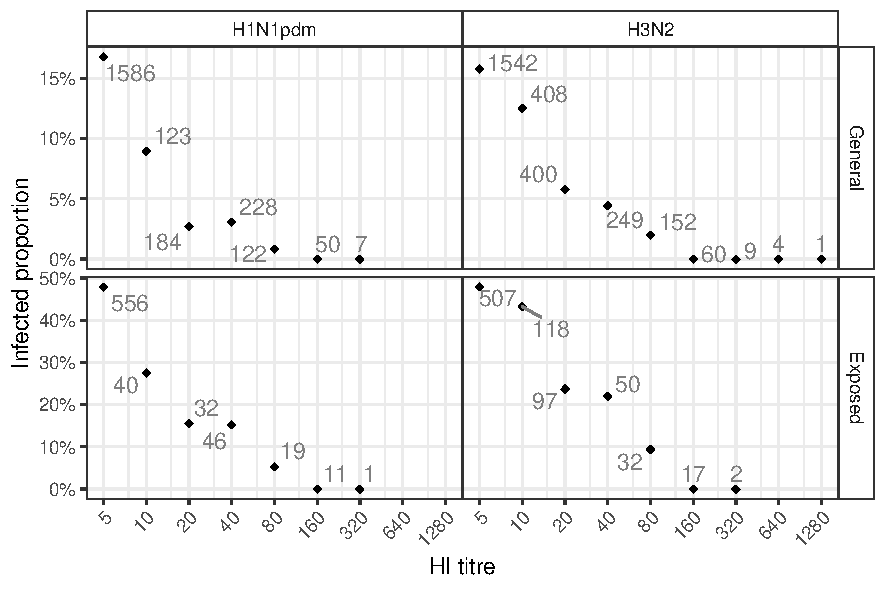
\includegraphics[width=0.9\textwidth]{../data-plot/hanam-hi-summ-light.pdf}
	\caption{
	Ha Nam cohort data. Subjects were grouped by virus and measured HI titre. Numbers next to points are the total number of observations in the corresponding group. The top row is all observations. The bottom row are the observations from households with at least one infection in a given season. The left column is observations for the H1N1pdm virus, the right row --- for H3N2 virus.
	}
	\label{HanamCounts}
\end{figure}

If baseline risk cannot justifiably be assumed to be 1, the fitted probability curve will be flatter than the true curve, thereby misrepresenting the true probability of infection across the titre range. An illustration is in Figure \ref{LogisticFit}. Thus, ignoring the baseline risk assumption will lead to biased estimates.


%\pagebreak

\begin{figure}[htp]
	\centering
	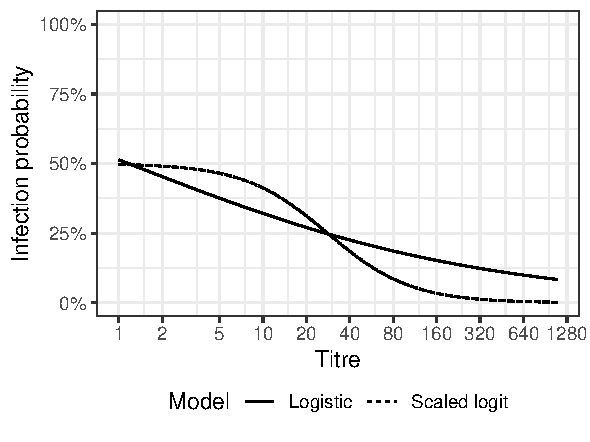
\includegraphics[width=0.6\textwidth]{../logistic-plot/lrex.pdf}
	\caption{
	An illustration of a bad fit of the logistic model. The dotted line (overlaps the dashed line) is the true probability curve $0.5\frac{\text{exp}(5 - 1.5 X_{\text{logtitre}})}{1 + \text{exp}(5 - 1.5 X_{\text{logtitre}})}$. The solid line is the expected fitted probability curve from standard logistic regression. The dashed line (overlaps the dotted line) is the expected fitted probability curve from scaled logistic regression. The expected curves was obtained from 10,000 simulations each with 10,000 observations simulated from the true curve. The models were fitted to each simulated dataset and the means of the regression estimates were taken from all simulations.
	}
	\label{LogisticFit}
\end{figure}
